\documentclass{article}
\usepackage[
paperwidth = 10cm, 
paperheight=10cm,
textwidth = 10cm,
textheight =10cm,
nohead,
nofoot,
nomarginpar,         
margin=0mm]{geometry}
\usepackage{amsmath,amsfonts,amssymb}
\usepackage{tikz,pgfplots}
\usetikzlibrary{arrows,arrows.meta,bending,calc,decorations,shadings,shadows,shapes,shapes.arrows,shapes.geometric}
\usetikzlibrary{calc,fadings,decorations.pathreplacing}
\usepgfplotslibrary{units,fillbetween,groupplots,colorbrewer}
\usetikzlibrary{pgfplots.colorbrewer,}
\usepackage{pgfplotstable}
\usetikzlibrary{3d,spy}
\usepgfmodule{plot}
\usepackage{scalerel}
\usepackage{graphicx}
\usepackage{tikz-dimline}
\usepackage{epstopdf}
\epstopdfsetup{outdir=out/,suffix=-generated}
\definecolor{As}{RGB}{255,255,0}
\definecolor{Al}{RGB}{173,216,230}
\definecolor{Ga}{RGB}{0,128,150}

\definecolor{background}{RGB}{77,77,77}

\definecolor{plane100}{RGB}{0,178,69}
\definecolor{plane010}{RGB}{0,255,208}

\newcommand*{\xMin}{0}%
\newcommand*{\xMax}{14}%
\newcommand*{\yMin}{-7}%
\newcommand*{\yMax}{0}%

\begin{document}
	\thispagestyle{empty}
\begin{tikzpicture}[remember picture,overlay]

	\shade[ball color=magenta, fill opacity=0.0,] (current page.center) circle [radius=1cm] node[scale=3,opacity=0,font=\bfseries](c0) {$\pmb{C_{2v}}$};


%---------------------- asymmetric in potential >
\draw ([xshift=-2.5cm]c0.west) circle [radius=1cm] node[anchor=center,text width=1.7cm] (c1){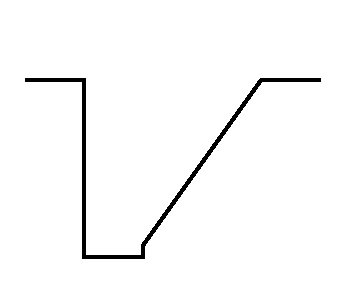
\includegraphics[width=\textwidth]{c2v-types/out/c2v-5}};
\def\arcu{-54}
\def\arcd{126}
\draw[inner sep=0mm, color=blue!60,right color=blue,middle
color=blue,opacity=0.5,] 
([xshift=-6mm]c0.south) to [bend right] ([xshift=6mm]c1.south) 
		arc (\arcu:\arcu+100:1) -- 
([xshift=6mm,yshift=16.5mm]c1.south) to [bend right] ([xshift=-6mm]c0.north) 
		arc (\arcd:\arcd+100:1);



\draw ([yshift=-3cm]c1.south) circle [radius=1cm] node[anchor=center,text width=1.7cm] (c11){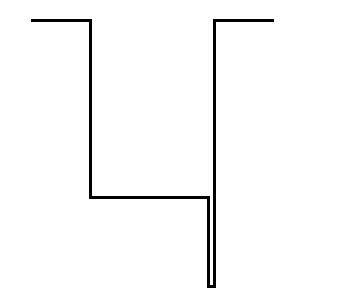
\includegraphics[width=\textwidth]{c2v-types/out/c2v-1}};

\def\ang{217}
\def\angd{38}
\draw[inner sep=0mm, color=green!60,right color=green,middle color=blue,opacity=0.5,] 
([xshift=-8mm,yshift=2.1mm]c1.south) arc (\ang:\ang+100:1)--
([xshift=8mm,yshift=2.1mm]c1.south) to [bend right] ([yshift=-2.1mm,xshift=-2mm]c11.north east) 
arc (\angd:\angd+100:1)--
([xshift=2mm,yshift=-2.1mm]c11.north west) to [bend right]  ([xshift=-8mm,yshift=2.1mm]c1.south);

 \draw ([yshift=3cm]c1.north) circle [radius=1cm] node[anchor=center,text width=1.7cm] (c12){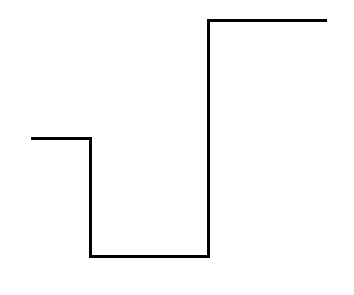
\includegraphics[width=\textwidth]{c2v-types/out/c2v-0}};
 \def\angcud{217}
 \def\angcudd{38}
\draw[inner sep=0mm, color=green!60,right color=green,middle color=blue,opacity=0.5,]
([xshift=-8mm,yshift=-2.1mm]c1.north) to [bend right] ([xshift=-8mm,yshift=2.1mm]c12.south) arc (\angcud:\angcud+100:1)--
([xshift=8mm,yshift=2.1mm]c12.south) to [bend right] ([xshift=8mm,yshift=-2.1mm]c1.north)
arc (\angcudd:\angcudd+100:1);

% \node[scale=1.25,blue,xshift=1mm,font=\bf] at (c12.north east){$\mathrm{(\!a_{1}\!)}$};
% \node[scale=1.25,blue,xshift=1mm,font=\bf] at (c11.north east){$\mathrm{(\!a_{2}\!)}$};
\node[scale=1.25,blue,xshift=1mm,font=\bf] at (c12.north east){(a)};
\node[scale=1.25,blue,xshift=1mm,font=\bf] at (c1.north east){(b)};
\node[scale=1.25,blue,xshift=1mm,font=\bf] at (c11.north east){(c)};


%-------------------------------- qws under strain ---------------------->

\draw ([yshift=3cm]c0.north) circle [radius=1cm] node[anchor=center,text width=1.7cm] (c2){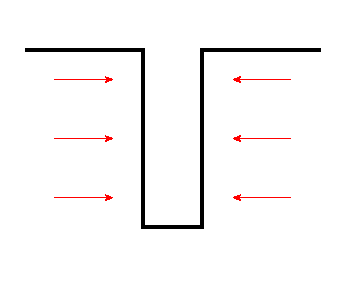
\includegraphics[width=\textwidth]{c2v-types/out/c2v-4}};

\def\arccu{217.5}
\def\arccd{36.5}
\draw[inner sep=0mm, color=blue!60,right color=blue,middle
color=blue,opacity=0.5,] 
 ([xshift=-8mm,yshift=-1.5mm]c0.north) to [bend right]  ([xshift=-8mm,yshift=2.1mm]c2.south) 
	arc (\arccu:\arccu+100:1) -- 
([xshift=8mm,yshift=2.1mm]c2.south) to [bend right] ([xshift=8mm,yshift=-2.1mm]c0.north)
 	arc (\arccd:\arccd+100:1);

	 \node[scale=1.25,blue,xshift=-1mm,font=\bf] at (c2.north west){(d)};


%--------------------------------- applied electric field -------------->

\draw ([yshift=-3cm]c0.south) circle [radius=1cm] node[anchor=center,text width=1.7cm] (c4){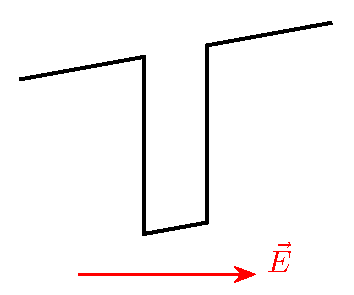
\includegraphics[width=\textwidth]{c2v-types/out/c2v-2}};

\def\arccccu{141}
\def\arccccd{323.5}
\draw[inner sep=0mm, color=blue!60,right color=blue,middle
color=blue,opacity=0.5,] 
([xshift=-8mm,yshift=1.5mm]c0.south) to [bend left]([xshift=-8mm,yshift=-2.1mm]c4.north) 
 arc (\arccccu:\arccccu-100:1)--
([xshift=8mm,yshift=-2.1mm]c4.north) to [bend left] ([xshift=8mm,yshift=2.1mm]c0.south)
arc (\arccccd:\arccccd-100:1);

\node[scale=1.25,blue,xshift=-1mm,font=\bf] at (c4.north west){(e)};




%------------------------- asymmetric double quantum wells --------------- >

\draw ([xshift=2.5cm]c0.east) circle [radius=1cm] node[anchor=center,text width=1.7cm] (c3){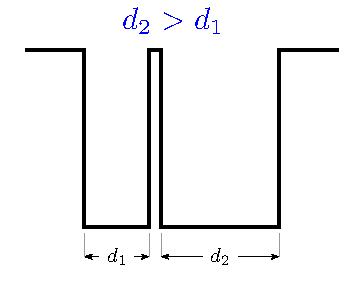
\includegraphics[width=\textwidth]{c2v-types/out/c2v-3}};
\def\arcccu{234}
\def\arcccd{53}

\draw[inner sep=0mm, color=blue!60,right color=blue,middle
color=blue,opacity=0.5,] 
 ([xshift=6mm,yshift=0mm]c0.south) to [bend left]  ([xshift=-6mm,yshift=0mm]c3.south) 
 arc (\arcccu:\arcccu-100:1) --
 ([xshift=-6mm,yshift=16.5mm]c3.south) to [bend left] ([xshift=6mm]c0.north) 
arc (\arcccd:\arcccd-100:1);

\node[scale=1.25,blue,xshift=-1mm,font=\bf] at (c3.north west){(f)};



\shade[ball color=cyan, fill opacity=0.8,] (current page.center) circle [radius=1cm] node[scale=3,opacity=1,font=\bfseries](c0) {$\pmb{C_{2v}}$};






\end{tikzpicture}
	
	


\end{document}